% Method overview for the ISBI 2027 version -- copied verbatim from
% paper/main.tex (Fig. 2 there, lines 772-797 and 801-945); edits are marked
% ISBI-EDIT. Panel (a) is paper/fig2_filmstrip.png, drawn by
% paper/make_filmstrip.py (A71_C1, its default), from
% benchmark/predictions/ours_23rec_topo (the released first-split model, which
% held that recording out).

% ----------------------------------------------------------
% Traced from real ground-truth masks -- training_data/masks/
% Sequence A71_C1, frames [0, 12, 24, 36, 48, 60, 72].  Generated by trace_masks.py;
% do not hand-edit.  Outlines are marching-squares contours of the
% annotated target; the skeleton is skimage.morphology.skeletonize.
% ----------------------------------------------------------
\newcommand{\neuronTight}{%
  \draw[mkfill] (-0.4418,-0.3361) -- (-0.4376,-0.2938) -- (-0.3826,-0.2642) -- (-0.3277,-0.2347) -- (-0.2621,-0.2156) -- (-0.2051,-0.1881) -- (-0.1649,-0.1438) -- (-0.1543,-0.1078) -- (-0.2135,-0.1332) -- (-0.2452,-0.1057) -- (-0.1818,-0.0846) -- (-0.1733,-0.0507) -- (-0.2262,-0.0190) -- (-0.2812,0.0106) -- (-0.3615,0.0148) -- (-0.4418,0.0106) -- (-0.4587,0.0486) -- (-0.3911,0.0486) -- (-0.3234,0.0486) -- (-0.2537,0.0338) -- (-0.1966,0.0063) -- (-0.1818,0.0676) -- (-0.1670,0.1374) -- (-0.1607,0.2072) -- (-0.1290,0.2051) -- (-0.1395,0.1311) -- (-0.1480,0.0550) -- (-0.1628,-0.0106) -- (-0.1205,-0.0528) -- (-0.0550,-0.0507) -- (0.0106,-0.0571) -- (0.0761,-0.0634) -- (0.1163,-0.0190) -- (0.1585,0.0233) -- (0.1628,0.0740) -- (0.1205,0.1163) -- (0.0972,0.1776) -- (0.0761,0.2410) -- (0.0507,0.3002) -- (0.0761,0.3129) -- (0.0994,0.2516) -- (0.1226,0.1903) -- (0.1522,0.1353) -- (0.1966,0.0951) -- (0.2558,0.0698) -- (0.3086,0.0381) -- (0.3573,0.0021) -- (0.4143,-0.0254) -- (0.4630,-0.0528) -- (0.4165,-0.0613) -- (0.3509,-0.0423) -- (0.3065,-0.0021) -- (0.2537,0.0296) -- (0.2072,-0.0042) -- (0.1881,-0.0698) -- (0.1374,-0.1036) -- (0.0698,-0.1205) -- (0.0063,-0.0994) -- (-0.0592,-0.0930) -- (-0.0972,-0.1395) -- (-0.0761,-0.2029) -- (-0.0592,-0.2706) -- (-0.0782,-0.2938) -- (-0.1036,-0.2347) -- (-0.1205,-0.1670) -- (-0.1607,-0.2114) -- (-0.1966,-0.2600) -- (-0.2516,-0.2473) -- (-0.3129,-0.2706) -- (-0.3657,-0.3023) -- (-0.4228,-0.3298);
}
\newcommand{\neuronTightSkel}{%
  \draw[mkskel] (-0.2347,-0.1226) -- (-0.2304,-0.1184) -- (-0.2262,-0.1184) -- (-0.2220,-0.1184) -- (-0.2177,-0.1184) -- (-0.2135,-0.1142) -- (-0.2093,-0.1099) -- (-0.2051,-0.1099) -- (-0.2008,-0.1099) -- (-0.1966,-0.1099) -- (-0.1924,-0.1057) -- (-0.1881,-0.1057) -- (-0.1839,-0.1015) -- (-0.1797,-0.0972) -- (-0.1755,-0.0972) -- (-0.1712,-0.0972) -- (-0.1670,-0.0972) -- (-0.1628,-0.0930) -- (-0.1585,-0.0930) -- (-0.1543,-0.0930) -- (-0.1501,-0.0930) -- (-0.1459,-0.0930) -- (-0.1416,-0.0930) -- (-0.1374,-0.0888) -- (-0.1332,-0.0846) -- (-0.1332,-0.0803) -- (-0.1332,-0.0761) -- (-0.1374,-0.0719) -- (-0.1374,-0.0676) -- (-0.1374,-0.0634) -- (-0.1416,-0.0592) -- (-0.1416,-0.0550) -- (-0.1459,-0.0507) -- (-0.1501,-0.0507) -- (-0.1543,-0.0465) -- (-0.1585,-0.0423) -- (-0.1628,-0.0381) -- (-0.1670,-0.0338) -- (-0.1712,-0.0296) -- (-0.1755,-0.0254) -- (-0.1755,-0.0211) -- (-0.1755,-0.0169) -- (-0.1797,-0.0127) -- (-0.1755,-0.0085) -- (-0.1755,-0.0042) -- (-0.1755,-0.0000) -- (-0.1755,0.0042) -- (-0.1755,0.0085) -- (-0.1755,0.0127) -- (-0.1755,0.0169) -- (-0.1712,0.0211) -- (-0.1712,0.0254) -- (-0.1712,0.0296) -- (-0.1712,0.0338) -- (-0.1712,0.0381) -- (-0.1712,0.0423) -- (-0.1670,0.0465) -- (-0.1670,0.0507) -- (-0.1670,0.0550) -- (-0.1670,0.0592) -- (-0.1670,0.0634) -- (-0.1628,0.0676) -- (-0.1628,0.0719) -- (-0.1628,0.0761) -- (-0.1628,0.0803) -- (-0.1628,0.0846) -- (-0.1628,0.0888) -- (-0.1628,0.0930) -- (-0.1628,0.0972) -- (-0.1628,0.1015) -- (-0.1628,0.1057) -- (-0.1585,0.1099) -- (-0.1585,0.1142) -- (-0.1585,0.1184) -- (-0.1585,0.1226) -- (-0.1543,0.1268) -- (-0.1543,0.1311) -- (-0.1543,0.1353) -- (-0.1501,0.1395) -- (-0.1501,0.1438) -- (-0.1501,0.1480) -- (-0.1501,0.1522) -- (-0.1501,0.1564) -- (-0.1501,0.1607) -- (-0.1459,0.1649) -- (-0.1459,0.1691) -- (-0.1459,0.1733) -- (-0.1459,0.1776) -- (-0.1459,0.1818) -- (-0.1459,0.1860) -- (-0.1459,0.1903) -- (-0.1459,0.1945) -- (-0.1459,0.1987) -- (-0.1459,0.2029) -- (-0.1459,0.2072) -- (-0.1459,0.2114) -- (-0.1459,0.2156);
  \draw[mkskel] (-0.1839,-0.0127) -- (-0.1881,-0.0127) -- (-0.1924,-0.0127) -- (-0.1966,-0.0085) -- (-0.2008,-0.0085) -- (-0.2051,-0.0085) -- (-0.2093,-0.0085) -- (-0.2135,-0.0042) -- (-0.2177,-0.0000) -- (-0.2220,-0.0000) -- (-0.2262,0.0042) -- (-0.2304,0.0042) -- (-0.2347,0.0085) -- (-0.2389,0.0085) -- (-0.2431,0.0127) -- (-0.2473,0.0127) -- (-0.2516,0.0169) -- (-0.2558,0.0211) -- (-0.2600,0.0211) -- (-0.2642,0.0211) -- (-0.2685,0.0254) -- (-0.2727,0.0254) -- (-0.2769,0.0254) -- (-0.2812,0.0296) -- (-0.2854,0.0296) -- (-0.2896,0.0296) -- (-0.2938,0.0296) -- (-0.2981,0.0296) -- (-0.3023,0.0296) -- (-0.3065,0.0296) -- (-0.3108,0.0338) -- (-0.3150,0.0338) -- (-0.3192,0.0338) -- (-0.3234,0.0338) -- (-0.3277,0.0338) -- (-0.3319,0.0338) -- (-0.3361,0.0338) -- (-0.3404,0.0338) -- (-0.3446,0.0338) -- (-0.3488,0.0338) -- (-0.3530,0.0338) -- (-0.3573,0.0338) -- (-0.3615,0.0338) -- (-0.3657,0.0338) -- (-0.3699,0.0338) -- (-0.3742,0.0338) -- (-0.3784,0.0296) -- (-0.3826,0.0296) -- (-0.3869,0.0296) -- (-0.3911,0.0296) -- (-0.3953,0.0296) -- (-0.3995,0.0296) -- (-0.4038,0.0296) -- (-0.4080,0.0296) -- (-0.4122,0.0296) -- (-0.4165,0.0296) -- (-0.4207,0.0296) -- (-0.4249,0.0296) -- (-0.4291,0.0296) -- (-0.4334,0.0296) -- (-0.4376,0.0296) -- (-0.4418,0.0296);
  \draw[mkskel] (-0.1290,-0.0846) -- (-0.1205,-0.0846) -- (-0.1120,-0.0846) -- (-0.1036,-0.0846) -- (-0.0951,-0.0803) -- (-0.0867,-0.0803) -- (-0.0782,-0.0761) -- (-0.0698,-0.0761) -- (-0.0613,-0.0719) -- (-0.0528,-0.0719) -- (-0.0444,-0.0676) -- (-0.0359,-0.0676) -- (-0.0275,-0.0676) -- (-0.0190,-0.0676) -- (-0.0106,-0.0719) -- (-0.0021,-0.0719) -- (0.0063,-0.0761) -- (0.0148,-0.0803) -- (0.0233,-0.0803) -- (0.0317,-0.0846) -- (0.0402,-0.0888) -- (0.0486,-0.0888) -- (0.0571,-0.0930) -- (0.0655,-0.0930) -- (0.0740,-0.0930) -- (0.0824,-0.0930) -- (0.0909,-0.0888) -- (0.0994,-0.0888) -- (0.1078,-0.0803) -- (0.1163,-0.0761) -- (0.1247,-0.0719) -- (0.1332,-0.0634) -- (0.1416,-0.0550) -- (0.1501,-0.0465) -- (0.1585,-0.0381) -- (0.1628,-0.0296) -- (0.1712,-0.0211) -- (0.1755,-0.0127) -- (0.1797,-0.0042) -- (0.1797,0.0042) -- (0.1881,0.0127) -- (0.1881,0.0211) -- (0.1881,0.0296) -- (0.1924,0.0381) -- (0.1966,0.0465) -- (0.1924,0.0550) -- (0.1924,0.0634) -- (0.1881,0.0719) -- (0.1839,0.0803) -- (0.1755,0.0888) -- (0.1670,0.0972) -- (0.1585,0.1057) -- (0.1501,0.1099) -- (0.1416,0.1184) -- (0.1332,0.1268) -- (0.1290,0.1353) -- (0.1247,0.1438) -- (0.1205,0.1522) -- (0.1163,0.1607) -- (0.1120,0.1691) -- (0.1120,0.1776) -- (0.1078,0.1860) -- (0.1036,0.1945) -- (0.1036,0.2029) -- (0.0994,0.2114) -- (0.0994,0.2199) -- (0.0951,0.2283) -- (0.0909,0.2368) -- (0.0867,0.2452) -- (0.0824,0.2537) -- (0.0782,0.2621) -- (0.0698,0.2706) -- (0.0655,0.2790) -- (0.0655,0.2875) -- (0.0655,0.2960) -- (0.0613,0.3044) -- (0.0655,0.3129) -- (0.0655,0.3213);
  \draw[mkskel] (0.2008,0.0507) -- (0.2051,0.0507) -- (0.2093,0.0507) -- (0.2135,0.0507) -- (0.2177,0.0507) -- (0.2220,0.0507) -- (0.2262,0.0507) -- (0.2304,0.0507) -- (0.2347,0.0507) -- (0.2389,0.0507) -- (0.2431,0.0507) -- (0.2473,0.0507) -- (0.2516,0.0507) -- (0.2558,0.0465) -- (0.2600,0.0465) -- (0.2642,0.0465) -- (0.2685,0.0423) -- (0.2727,0.0423) -- (0.2769,0.0423) -- (0.2812,0.0423) -- (0.2854,0.0381) -- (0.2896,0.0338) -- (0.2938,0.0296) -- (0.2981,0.0254) -- (0.3023,0.0254) -- (0.3065,0.0211) -- (0.3108,0.0169) -- (0.3150,0.0127) -- (0.3192,0.0085) -- (0.3234,0.0042) -- (0.3277,-0.0000) -- (0.3319,-0.0042) -- (0.3361,-0.0042) -- (0.3404,-0.0085) -- (0.3446,-0.0085) -- (0.3488,-0.0127) -- (0.3530,-0.0169) -- (0.3573,-0.0211) -- (0.3615,-0.0254) -- (0.3657,-0.0296) -- (0.3699,-0.0296) -- (0.3742,-0.0338) -- (0.3784,-0.0338) -- (0.3826,-0.0338) -- (0.3869,-0.0381) -- (0.3911,-0.0381) -- (0.3953,-0.0381) -- (0.3995,-0.0381) -- (0.4038,-0.0381) -- (0.4080,-0.0381) -- (0.4122,-0.0423) -- (0.4165,-0.0423) -- (0.4207,-0.0423) -- (0.4249,-0.0465) -- (0.4291,-0.0465) -- (0.4334,-0.0465) -- (0.4376,-0.0507) -- (0.4418,-0.0550) -- (0.4461,-0.0550) -- (0.4503,-0.0592) -- (0.4545,-0.0592);
  \draw[mkskel] (-0.1120,-0.0888) -- (-0.1120,-0.0930) -- (-0.1120,-0.0972) -- (-0.1163,-0.1015) -- (-0.1163,-0.1057) -- (-0.1163,-0.1099) -- (-0.1163,-0.1142) -- (-0.1163,-0.1184) -- (-0.1163,-0.1226) -- (-0.1163,-0.1268) -- (-0.1163,-0.1311) -- (-0.1205,-0.1353) -- (-0.1205,-0.1395) -- (-0.1205,-0.1438) -- (-0.1247,-0.1480) -- (-0.1290,-0.1480) -- (-0.1332,-0.1480) -- (-0.1374,-0.1522) -- (-0.1416,-0.1522) -- (-0.1459,-0.1564) -- (-0.1501,-0.1607) -- (-0.1501,-0.1649) -- (-0.1543,-0.1691) -- (-0.1585,-0.1733) -- (-0.1585,-0.1776) -- (-0.1628,-0.1818) -- (-0.1670,-0.1860) -- (-0.1712,-0.1903) -- (-0.1755,-0.1945) -- (-0.1797,-0.1987) -- (-0.1839,-0.2029) -- (-0.1881,-0.2072) -- (-0.1881,-0.2114) -- (-0.1924,-0.2156) -- (-0.1966,-0.2199) -- (-0.2008,-0.2199) -- (-0.2051,-0.2199) -- (-0.2093,-0.2199) -- (-0.2135,-0.2199) -- (-0.2177,-0.2199) -- (-0.2220,-0.2241) -- (-0.2262,-0.2241) -- (-0.2304,-0.2241) -- (-0.2347,-0.2241) -- (-0.2389,-0.2241) -- (-0.2431,-0.2241) -- (-0.2473,-0.2241) -- (-0.2516,-0.2283) -- (-0.2558,-0.2283) -- (-0.2600,-0.2283) -- (-0.2642,-0.2325) -- (-0.2685,-0.2325) -- (-0.2727,-0.2368) -- (-0.2769,-0.2368) -- (-0.2812,-0.2368) -- (-0.2854,-0.2410) -- (-0.2896,-0.2410) -- (-0.2938,-0.2410) -- (-0.2981,-0.2410) -- (-0.3023,-0.2452) -- (-0.3065,-0.2452) -- (-0.3108,-0.2495) -- (-0.3150,-0.2495) -- (-0.3192,-0.2537) -- (-0.3234,-0.2537) -- (-0.3277,-0.2579) -- (-0.3319,-0.2579) -- (-0.3361,-0.2621) -- (-0.3404,-0.2621) -- (-0.3446,-0.2664) -- (-0.3488,-0.2706) -- (-0.3530,-0.2706) -- (-0.3573,-0.2748) -- (-0.3615,-0.2748) -- (-0.3657,-0.2790) -- (-0.3699,-0.2833) -- (-0.3742,-0.2833) -- (-0.3784,-0.2875) -- (-0.3826,-0.2875) -- (-0.3869,-0.2875) -- (-0.3911,-0.2875) -- (-0.3953,-0.2917) -- (-0.3995,-0.2917) -- (-0.4038,-0.2917) -- (-0.4080,-0.2960) -- (-0.4122,-0.3002) -- (-0.4165,-0.3044) -- (-0.4207,-0.3044) -- (-0.4249,-0.3086) -- (-0.4291,-0.3129) -- (-0.4334,-0.3171) -- (-0.4376,-0.3213) -- (-0.4418,-0.3213) -- (-0.4461,-0.3256);
  \draw[mkskel] (-0.1205,-0.1480) -- (-0.1163,-0.1522) -- (-0.1120,-0.1564) -- (-0.1078,-0.1564) -- (-0.1036,-0.1607) -- (-0.1036,-0.1649) -- (-0.1036,-0.1691) -- (-0.1036,-0.1733) -- (-0.0994,-0.1776) -- (-0.0994,-0.1818) -- (-0.0994,-0.1860) -- (-0.0994,-0.1903) -- (-0.0951,-0.1945) -- (-0.0951,-0.1987) -- (-0.0951,-0.2029) -- (-0.0951,-0.2072) -- (-0.0909,-0.2114) -- (-0.0909,-0.2156) -- (-0.0909,-0.2199) -- (-0.0867,-0.2241) -- (-0.0867,-0.2283) -- (-0.0867,-0.2325) -- (-0.0824,-0.2368) -- (-0.0824,-0.2410) -- (-0.0824,-0.2452) -- (-0.0782,-0.2495) -- (-0.0782,-0.2537) -- (-0.0782,-0.2579) -- (-0.0782,-0.2621) -- (-0.0740,-0.2664) -- (-0.0740,-0.2706) -- (-0.0698,-0.2748) -- (-0.0698,-0.2790) -- (-0.0698,-0.2833) -- (-0.0655,-0.2875) -- (-0.0655,-0.2917) -- (-0.0613,-0.2960) -- (-0.0613,-0.3002) -- (-0.0613,-0.3044);
}
% skeleton 513 px vs 4977 mask px -> skeleton is 10.3\% of the mask

% framed panel holding a traced mask: #1 x, #2 y, #3 half-size, #4 macro
\newcommand{\maskpanel}[4]{%
  \begin{scope}[shift={(#1,#2)}]
    \draw[black!35, line width=0.35pt, fill=white] (-#3,-#3) rectangle (#3,#3);
    \begin{scope}[scale={2*#3}]#4\end{scope}
  \end{scope}
}

\begin{tikzpicture}[
  font=\small,
  rule/.style={draw=black!45, line width=0.4pt},
  plab/.style={font=\bfseries\small, text=black, anchor=north west},
  ptit/.style={font=\small, text=black, anchor=north west},
  note/.style={font=\scriptsize, text=black!60, align=left},
  sm/.style={font=\fontsize{6.4}{7.4}\selectfont, text=black!60},
  bx/.style={rounded corners=1pt, align=center, inner sep=2.5pt,
             line width=0.5pt, font=\fontsize{7}{8}\selectfont},
  frz/.style={bx, fill=black!5,    draw=black!45},
  lra/.style={bx, fill=ourblue!10, draw=ourblue!75},
  trn/.style={bx, fill=teal!10,    draw=teal!75},
  ar/.style={-{Stealth[length=1.7mm,width=1.4mm]}, draw=black!65, line width=0.5pt},
  loop/.style={-{Stealth[length=1.7mm,width=1.4mm]}, draw=amber!85!black,
               line width=0.7pt},
  grad/.style={-{Stealth[length=1.7mm,width=1.4mm]}, draw=crimson!85,
               line width=0.6pt},
  mkfill/.style={fill=mk!25, draw=mk!90!black, line width=0.25pt},
  mkskel/.style={draw=mk2, line width=0.4pt, line cap=round},
  nd/.style={circle, draw=black!60, fill=white, line width=0.5pt,
             minimum size=0.26cm, inner sep=0pt},
]

% ==================  (a)  the propagation task  ==================
\node[plab] at (0.00,7.55) {(a)};
\node[ptit] at (0.62,7.55)
     {One annotation at $t=0$ propagates through the whole recording};

% Real phase contrast: the frame-0 ground-truth prompt (navy) and the model's
% own propagated masks (teal).  Seven 1.24 cm cells on a 2.30 cm pitch, 50 um
% scale bar burnt into the last cell.  Built by make_filmstrip.py, which
% refuses to draw a recording the model trained on, and refuses to draw at all
% unless the stack re-scores to the IoU in results/test/ours_23rec_topo.csv.
\node[anchor=south west, inner sep=0] at (0.53,5.80)
     {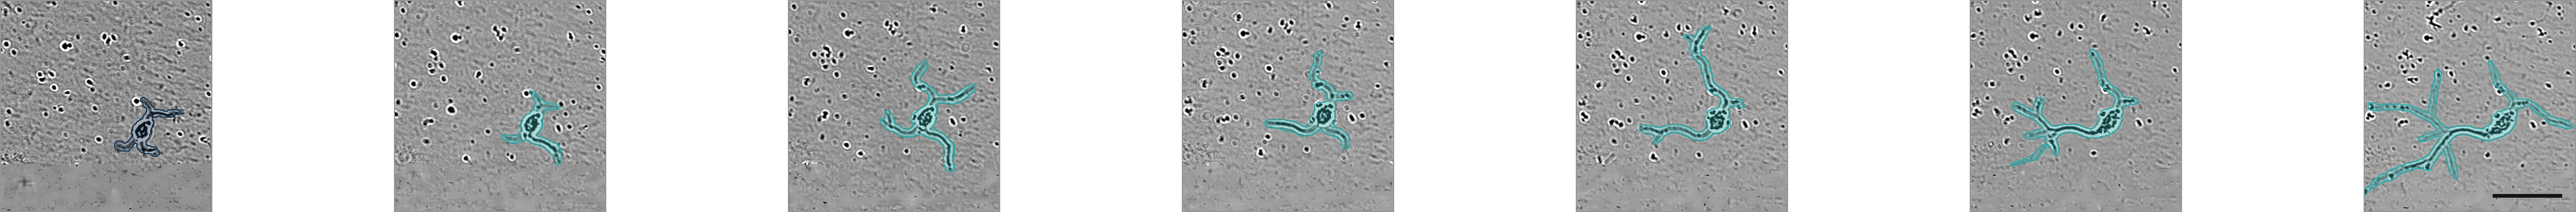
\includegraphics[width=15.04cm]{fig2_filmstrip}};

\draw[rule] (0.90,5.70) -- (15.35,5.70);
\foreach \x in {1.15,3.45,5.75,8.05,10.35,12.65,14.95}
  \draw[rule] (\x,5.70) -- (\x,5.60);
\foreach \x/\lb in {1.15/0, 3.45/12, 5.75/24, 8.05/36, 10.35/48, 12.65/60,
                    14.95/72}
  \node[sm, anchor=north] at (\x,5.56) {\lb};
\node[sm, anchor=west] at (15.45,5.64) {h};
\node[sm, text=navy, anchor=north] at (1.15,5.26) {given};
\node[sm, anchor=north east] at (16.20,5.26) {scale bar $50\,\mu$m};
\node[sm, anchor=north] at (9.20,5.26)
     {propagated with no further prompt, correction or re-initialization};

\draw[rule] (0,4.88) -- (16.20,4.88);

% ==================  (b)  where the model is adapted  ============
\node[plab] at (0.00,4.68) {(b)};
\node[ptit] at (0.62,4.68) {Adaptation sites};
\node[note, anchor=north west] at (0.62,4.32)
     {$5{,}557{,}250$ of $39{,}876{,}930$ parameters trainable ($13.9\,\%$)};

\node[frz, minimum width=2.30cm, minimum height=0.74cm, anchor=west] (enc)
     at (0.10,3.35) {Image encoder\\{\fontsize{6}{7}\selectfont Hiera-tiny}};
\node[lra, minimum width=1.70cm, minimum height=0.74cm, anchor=west] (hier)
     at (2.85,3.35) {blocks 10--11\\{\fontsize{6}{7}\selectfont $r{=}8$}};
\node[trn, minimum width=2.10cm, minimum height=0.74cm, anchor=west] (pe)
     at (6.10,3.35) {Prompt encoder\\{\fontsize{6}{7}\selectfont frame-0 mask}};

\node[lra, minimum width=2.55cm, minimum height=0.80cm, anchor=west] (mem)
     at (0.10,1.95) {Memory attention\\{\fontsize{6}{7}\selectfont $r{=}16$,
       40 sites}};
\node[lra, minimum width=2.55cm, minimum height=0.80cm, anchor=west] (dec)
     at (3.30,1.95) {Mask decoder\\{\fontsize{6}{7}\selectfont $r{=}16$,
       28 sites}};
\node[trn, minimum width=2.90cm, minimum height=0.50cm, anchor=west] (menc)
     at (2.00,0.72) {Memory encoder $+$ bank};

\draw[ar] (enc.east) -- (hier.west);
\draw[ar] (hier.south) -- ++(0,-0.26) -| (mem.north);
\draw[ar] (mem.east) -- (dec.west);
\draw[ar] (pe.south) -- ++(0,-0.42) -| ([xshift=8mm]dec.north);
\draw[ar] (dec.east) -- ++(0.24,0) node[right, sm, text=black] {$\hat{m}_t$};
\draw[loop] (dec.south) -- (dec.south |- menc.north);
\draw[loop] (menc.west) -| (mem.south);
\node[sm, text=amber!55!black, anchor=west] at (0.10,0.18)
     {the bank read at $t$ holds the mask predicted at $t-1$};

% --- key
\begin{scope}[shift={(0.10,-0.30)}]
  \node[frz, minimum width=0.26cm, minimum height=0.17cm, anchor=west] at (0,0) {};
  \node[sm, anchor=west, text=black] at (0.32,0) {frozen};
  \node[lra, minimum width=0.26cm, minimum height=0.17cm, anchor=west] at (1.25,0) {};
  \node[sm, anchor=west, text=black] at (1.57,0) {LoRA-adapted, $0.91$\,M};
  \node[trn, minimum width=0.26cm, minimum height=0.17cm, anchor=west] at (4.45,0) {};
  \node[sm, anchor=west, text=black] at (4.77,0) {trained directly, $4.64$\,M};
\end{scope}

% ==================  (c)  the objective  =========================
\draw[rule] (9.10,4.68) -- (9.10,-0.50);

\node[plab] at (9.35,4.68) {(c)};
\node[ptit] at (9.97,4.68) {Objective};
\node[note, anchor=north west] at (9.97,4.32)
     {16-frame clips, bank not detached};

\node[sm, anchor=south] at (12.40,3.58) {memory writes};
\node[nd] (n0) at (10.15,3.42) {};
\node[nd] (n1) at (11.35,3.42) {};
\node[nd] (n2) at (12.55,3.42) {};
\node[nd] (n3) at (14.75,3.42) {};
\node[sm] at (13.65,3.42) {$\cdots$};
\draw[ar] (n0) -- (n1);
\draw[ar] (n1) -- (n2);
\draw[ar] (n2) -- (13.30,3.42);
\draw[ar] (14.00,3.42) -- (n3);
\foreach \x/\lb in {10.15/t, 11.35/{t{+}1}, 12.55/{t{+}2}, 14.75/{t{+}15}}
  \node[sm, anchor=north] at (\x,3.18) {$\lb$};

\draw[grad] (14.75,2.92) .. controls (13.80,2.46) and (11.10,2.46) .. (10.15,2.92);
\node[sm, text=crimson!85, anchor=north] at (12.45,2.50)
     {gradient retained back to the start of the clip};

% --- the composite loss, as a ruled table
\draw[rule] (9.35,2.02) -- (16.20,2.02);
\node[sm, anchor=west] at (9.42,1.86) {weight};
\node[sm, anchor=west] at (10.42,1.86) {term};
\node[sm, anchor=west] at (12.30,1.86) {compares};
\draw[rule] (9.35,1.72) -- (16.20,1.72);
\foreach \y/\w/\t/\c in {1.52/{$3.0$}/{Focal}/{pixels},
                         1.22/{$2.0$}/{Dice}/{regions}}{
  \node[font=\fontsize{6.8}{7.8}\selectfont, anchor=west] at (9.42,\y) {\w};
  \node[font=\fontsize{6.8}{7.8}\selectfont, anchor=west] at (10.42,\y) {\t};
  \node[sm, anchor=west] at (12.30,\y) {\c};
}
\foreach \y/\w/\t/\c in {0.92/{$0.3$}/{cbDice}/{centerlines},
                         0.62/{$0.3$}/{Supervoxel}/{connected components}}{
  \node[font=\fontsize{6.8}{7.8}\selectfont, text=ourblue, anchor=west] at (9.42,\y) {\w};
  \node[font=\fontsize{6.8}{7.8}\selectfont, text=ourblue, anchor=west] at (10.42,\y) {\t};
  \node[sm, text=ourblue!85!black, anchor=west] at (12.30,\y) {\c};
}
\draw[rule] (9.35,0.44) -- (16.20,0.44);

% --- what the two topology terms actually look at
\colorlet{mk}{black!45}\colorlet{mk2}{ourblue}
\maskpanel{9.78}{-0.06}{0.36}{\neuronTight\neuronTightSkel}
% ISBI-EDIT: the long paper's note ("a severed branch is invisible to an area
% term and costly to a centerline term") is dropped -- paper/main.tex records
% (Discussion, caution b) that cbDice tracks IoU to within 0.02 when branches
% are deleted, so the sensitivity claim has no measurement behind it. What is
% kept is measured: skeleton 513 px vs 4977 mask px on this frame.
\node[sm, anchor=west, align=left] at (10.30,-0.06)
     {held-out target, skeleton in blue:\\
      cbDice weights thin branches; the supervoxel\\
      term catches cuts and bridges};

\end{tikzpicture}
